\documentclass{mipt-thesis-bs}
%\documentclass[a4paper,14pt]{report}
\usepackage{mipt-thesis-bs}

% Следующие две строки нужны только для biblatex. Для inline-библиографии их следует убрать.
%\usepackage{mipt-thesis-biblatex}
%\addbibresource{thesis-bibliography.bib}
\bibliography{thesis-bibliography}
\newcommand{\argmin}{\mathop{\mathrm{argmin}}}


\begin{document}
\setcounter{page}{2}
\chapter{Аннотация}
%\section{Аннотация}
Алгоритмы нейрокомпьютерных интерфейсов решают задачу преобразования сигналов нейронов головного мозга в команды исполняющей системы. В данной работе исследуются механизмы регуляции движения конечностей нейронами головного мозга. Сложность данной задачи заключается в избыточной размерности сигнала. Высокая размерность признакового пространства сигналов приводит к неустойчивости модели машинного обучения. Задачей данной работы является снижение размерности входных данных алгоритма через построение удобного признакового пространства.

Сигнал высокой размерности предлагается аппроксимировать локальной моделью, что существенно уменьшает размерность пространства параметров. В дальнейшем, пространство параметров локальной модели используется в качестве признакового пространства. Таким образом, результирующая модель становится проще и устойчивее. При решении задачи используются данные электрокортикограмм, собранные на основе исследований активности нейронов головного мозга обезьян.
В результате проведенных исследований было получено несколько локальных моделей, сокращающих размерность пространства признаков в N раз и упрощающих вычисления результирующей модели.


\newpage
\tableofcontents{}


\chapter{Введение}
В последнее время большое количество работ посвящено методам считывания мозговой активности и декодирования информации \cite{Hu2018,Song2017,Loza2017,Eliseyev2016,Gaglianese2016,Bundy2016,Morishita2014}.
Основным приложением данных методов являются нейрокомпьютерные интерфейсы (Brain Computer Interface), которые позволяют восстановить мобильность людей с нарушениями двигательных функций.  Алгоритм BCI транслирует сигналы нейронов головного мозга в команды для исполняющей системы \cite{Morishita2014}. Это дает возможность регулировать движение роботизированной конечности в соответствии с механизмами нервной регуляции. \cite{Donoghue2008}. 

В этой работе используются данные сигналов мозга, полученные инвазивным методом электрокортикографии (subdural ECoG) \cite{Sirven2014}. Сложность задачи декодирования сигналов мозга заключается в избыточной размерности пространства признаков: модель прогнозирования намерений является неустойчивой. Для построения устойчивой модели необходимо построить удобное признаковое пространство.

Исследование состоит в восстановлении зависимостей между сигналами ECoG и движениями конечностей. Для точного предсказания траектории движения в трехмерном пространстве требуется снизить размерность исходного признакового пространства.

Стандартные подходы для установления зависимостей между электрокортикограммой и координатами конечностей состоят в извлечении информативных признаков из пространственных, частотных и временных характеристик сигнала\cite{Morishita2014,Alexander2013}. Большинство методов в смежных работах исследуют только частотные характеристики\cite{Chin2007,Eliseyev2014,Loza2017}. В работах \cite{Eliseyev2016,Motrenko2018} рассматриваются все признаки вне зависимости от их природы. Наиболее распространёнными моделями для предсказания движения являются алгоритмы PLS\cite{Rosipal2006,Eliseyev2016} и PCA\cite{Zhao2010,Song2017}. В работе \cite{Zhao2014} используются алгоритмы, построенные на скрытых марковских моделях. В  работах \cite{Loza2017,Song2017} авторы рассматривают различные участки сигнала в виде слов. В работе \cite{Motrenko2018} исследован метод отбора признаков с помощью квадратичного программирования (Quadratic Programming Feature Selection \cite{rodriguez2010quadratic}).

В данной работе для моделирования фронта распределения сигнала предлагается использовать локальную структуру сигнала. Движение фронта возбуждения нейронов приближается с помощью локальной модели прогнозирования движений, а в качестве нового признакового описания объектов используются параметры построенной локальной модели. Полученный  метод значительно снижает размерность данных, использует пространственную информацию и сохраняет свойства распространения сигнала.
Как следствие, количество параметров конечной модели значительно уменьшается. Получается более простая аппроксимация сигнала высокой размерности и более устойчивая прогностическая модель.

\chapter{Постановка задачи}
\section{Нейробиологические предпосылки некоторых гипотез}
В данной работе для моделирования фронта распределения сигнала предлагается использовать локальную структуру сигнала. Нейроны и связи между ними образуют граф, описывающий возможные пути распространения сигналов. Каждый нейрон соединен с помощью множества отростков с приблизительно 20 тысячами других нейронов. Точно учесть локальную структуру графа при описании сигнала невозможно, так как это потребует большого количества вычислительных ресурсов. В связи с этим предлагается модель локальной аппроксимации формы и перемещения фронта. Активность нейронов представляет собой временные вспышки сигналов различной интенсивности, их суперпозицию и распространение. Каждый канал имеет доступ к сигналам некоторого количества нейронов, находящихся в небольшой области пространства и снимает суммарную интенсивность сигнала.  

\begin{figure}
\begin{center}
	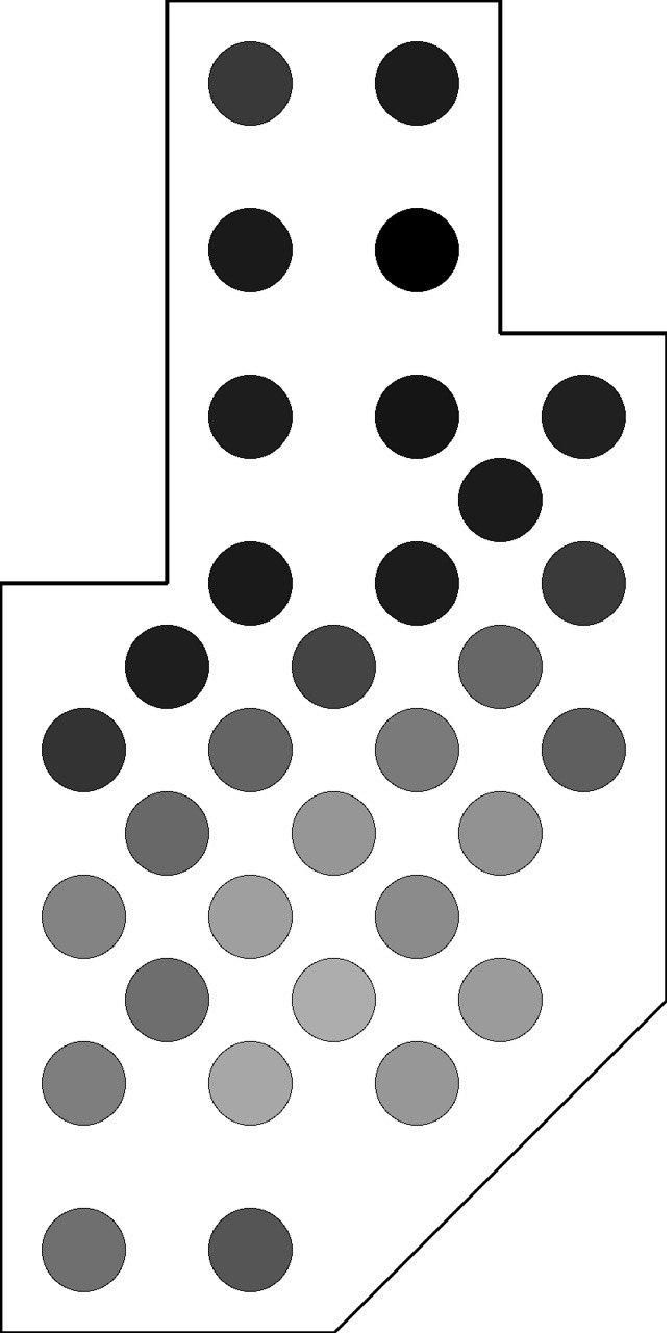
\includegraphics[width=45pt,height=\textheight,keepaspectratio]{imgs/wave0.pdf}
	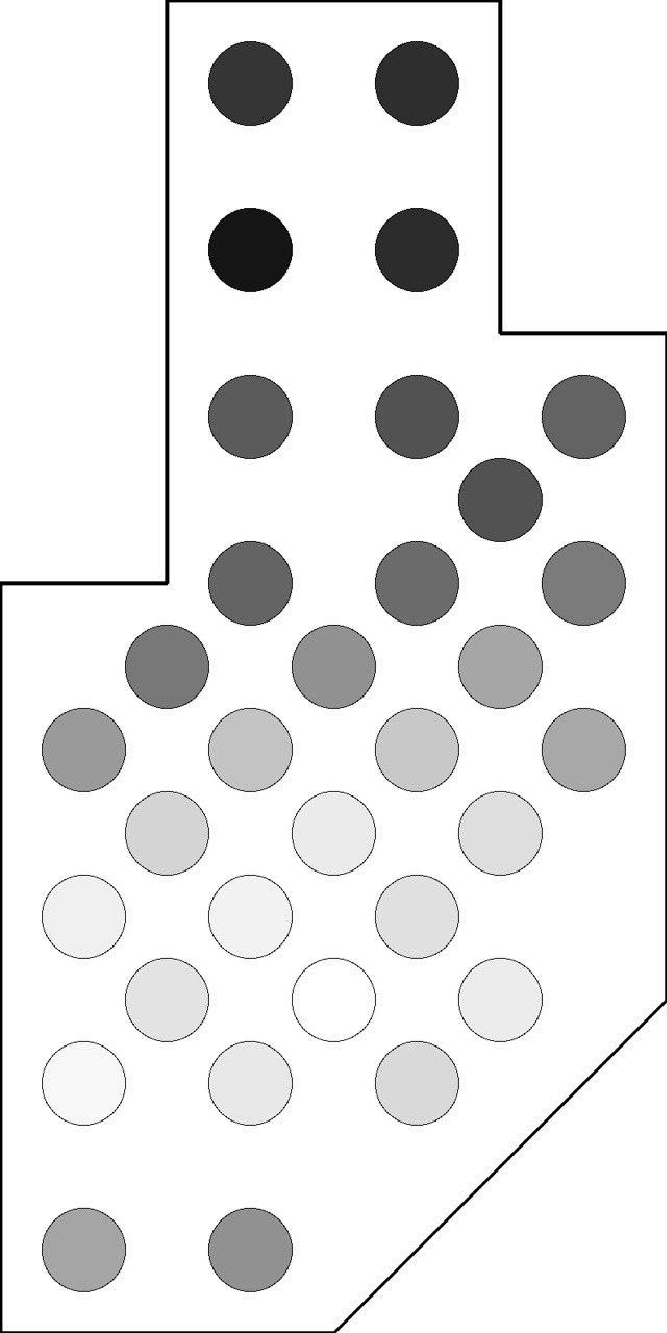
\includegraphics[width=45pt,height=\textheight,keepaspectratio]{imgs/wave1.pdf}
	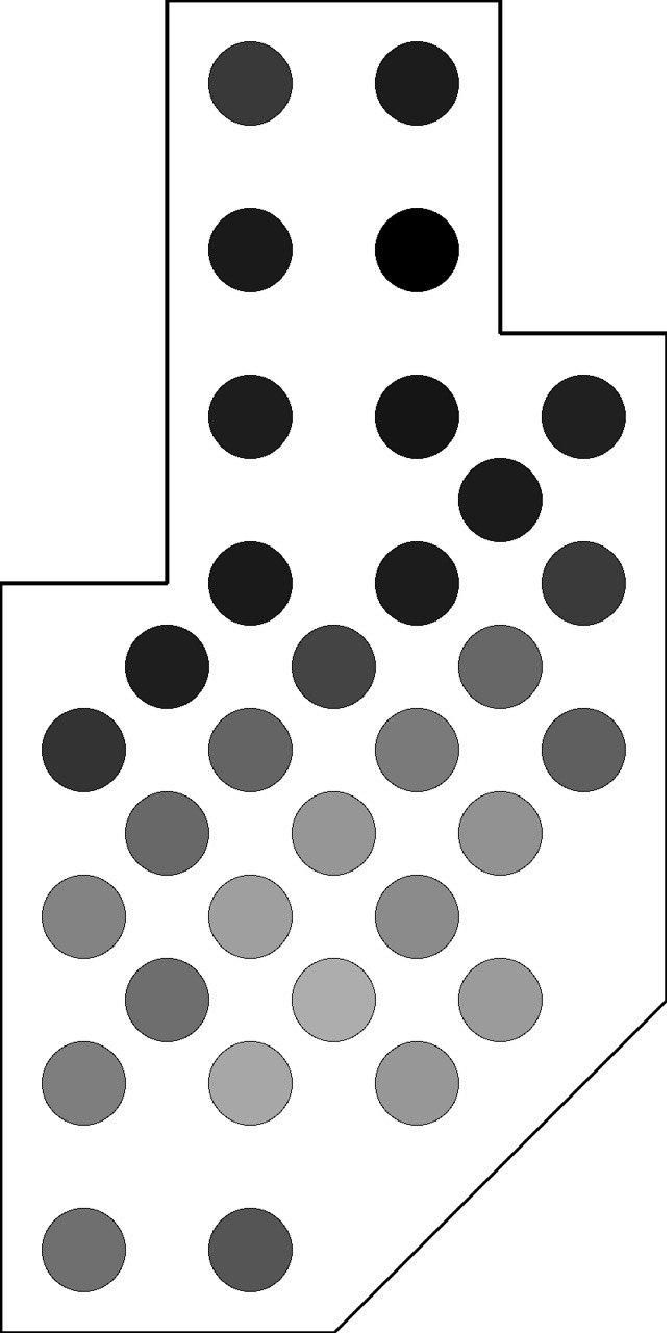
\includegraphics[width=45pt,height=\textheight,keepaspectratio]{imgs/wave0.pdf}
	\caption{Перемещение сигнала среди каналов}	
	\label{fig:waves}
	\end{center}
\end{figure}

На [рис.1] можно заметить, что фронт перемещается по сети в большинстве случаев как единое целое, при этом интенсивность сигнала максимальна в центре множества активных узлов и убывает к периферии. У такой структуры сигнала есть возможное объяснение, основанное на устройстве нейронной сети. Нейрон имеет большое количество небольших отростков - дендритов, основной функцией которых является передача возбуждения к телу нейрона извне, и обычно один аксон, служащий для передачи импульса от тела другим нейронам или мышечной ткани. Получается, что импульсы собираются от периферии к центру каждого нейрона, после чего суммарный импульс, если он достаточно велик, передается по аксону дальше. Таким образом, движение фронта возбуждения приближается с помощью локальной модели прогнозирования движений. В качестве признакового описания объектов используются параметры построенной локальной модели.

Предлагается рассматривать в первую очередь распределения сигнала в пространстве в каждый момент времени. В каждый момент времени рассчитываются параметры модели. Рассматриваются гипотезы двумерных нормального и гамма распределений. Также предлагаются локальные модели, основывающиеся на временных отрезках данных. Исходный сигнал разбивается на отрезки \textbf{и что-то дальше происходит}

Полученные  методы снижают размерность данных, используют пространственную информацию и сохраняют свойства распространения сигнала.

\section{Данные}

В эксперименте используются данные с сайта neurotycho.org. Сбор данных производился с использованием методики Multi-Dimensional Recording. Запись сигналов ECoG и траектории движения руки проводилась одновременно. Каждый из экспериментов длился 15 минут, первые 8 минут производилась запись обучающей выборки, оставшиеся 7 минут~– запись тестовой выборки. На [рис.2] приведен пример записи ECoG с некоторых каналов.

\begin{figure}
\begin{center}
	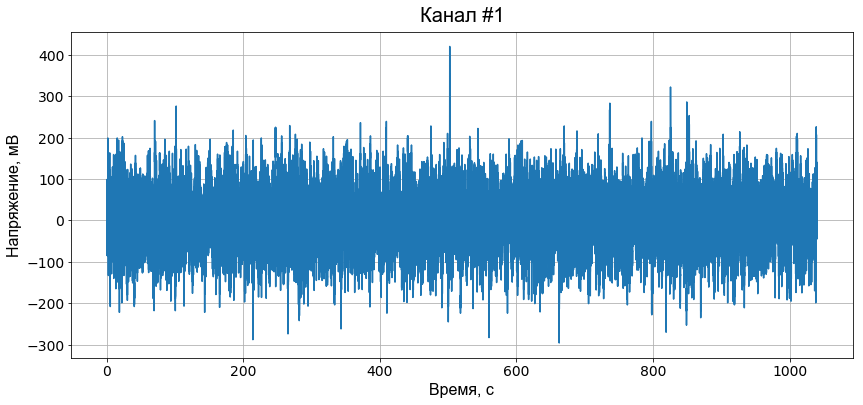
\includegraphics[width=300pt,height=\textheight,keepaspectratio]{imgs/Raw_ch1.png}
	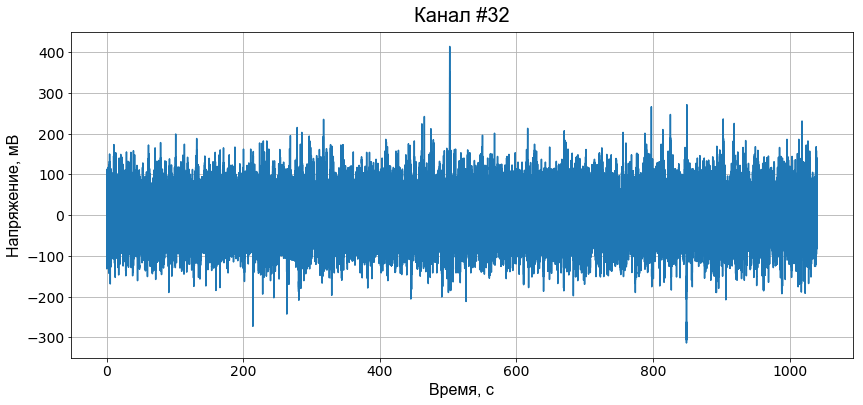
\includegraphics[width=300pt,height=\textheight,keepaspectratio]{imgs/Raw_ch32.png}
	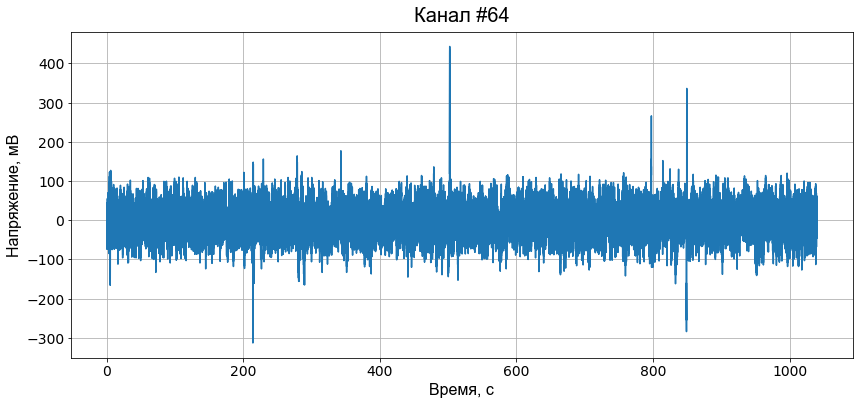
\includegraphics[width=300pt,height=\textheight,keepaspectratio]{imgs/Raw_ch64.png}
	\caption{Изменения значений напряжения на 1, 32 и 64 каналах}	
	\label{fig:raw}
	\end{center}
\end{figure}

Исходные данные представляют собой отрезки многомерных временных рядов электрокортикограммы. Запись электрокортикограммы производилась с частотой 1 кГц, запись движения - с частотой 120 Гц.
Рассматривалась синхронизация движения двумя методами: 
\begin{enumerate}
\item каждой координате было сопоставлено значение ECoG, соответствующее временной отметке движения
\item каждой координате было сопоставлено значение ECoG, полученное экспоненциальным сглаживанием значений за последние 0.007 с. 0.007 с - среднее занчение временного промежутка между соседними отметками времени координат
\end{enumerate}

Пространство исходных данных имеет размерность $T \times N$. Пространство данных, на которых обучается большинство моделей, в частности \cite{Motrenko 2018} - результат предобработки исходных данных, оно имеет размерность $T \times N \times F$, где $N$ – число каналов, $T$ – количество отсчетов времени, $F$ – дискретный спектр наблюдаемых частот. Тогда матрица значений напряжения $\mathbf{X} \in \mathbb{R}^{T \times (N \circ F)}$, целевая переменная - $\mathbf{Y} \in \mathbb{R}^{T \times 3}$. \\


Исходные данные представлены в виде массивов:
\begin{equation}
\mathbf{X} = \{x_{ti}\}_{\substack{t=1,\dots,T,\\ i=1,\dots,N;}};
\end{equation} 
\begin{equation}
\mathbf{Y} = \{y_{ti}\}_{\substack{t=1,\dots,T,\\ i=1,2,3;}};
\end{equation}

Объектом будем называть вектор $\mathbf{x}_t \in \mathbb{R}^{N}$ c измерениями в каждый отрезок времени, $i = 1,\dots,T$. Вектор состоит из $N$ элементов, каждый из которых соответствует каналу. Значение $y_{ti}$ отвечает $i$-й координате траектории движения конечности в момент времени $t$.\\

\section{Задача}
Необходимо построить информативное признаковое пространство для предсказания траектории движения конечности. Модель прогнозирования $f:\mathbf{X}\to\mathbf{Y}$ предлагается искать классе суперпозиции двух моделей: $f = g \circ h:$ $\mathbf{X}\to\mathbf{Y}$. Локальная модель $g:\mathbf{X}\times\mathbf{\theta}\to\mathbf{X}$ использует локальную пространственную структуру сигнала для аппроксимации перемещения фронта возбуждения.
 %Примером локальной модели является модель %авторегрессии:
%\begin{equation}
%\left(\begin{array}{@{}c|ccc@{}}
%x_{t+1,i} & x_{t,i}   & \cdots & x_{t-d,i}   \%\
%x_{t,i}   & x_{t-1,i} & \cdots & x_{t-d-1,i} \%\
%\cdots     & \cdots     & \cdots & \cdots	\\
%x_{T_{i},i}   & \cdots     & \cdots & \cdots   %\\
%\end{array}\right)
%\begin{pmatrix}
%\theta_1^{i} \\
%\theta_2^{i} \\
%\cdots \\
%\theta_d^{i}
%\end{pmatrix}.
%\end{equation}
Модель $g(\mathbf{X}, \mathbf{\theta})$ решает задачу оптимизации параметров $\mathbf{\theta}^{i}$ для временного ряда $\mathbf{x_{i}}$:
\begin{equation}
\mathbf{\theta}^i(\mathbf{X}) = \argmin_{\mathbf{\theta}^i} L(g(\mathbf{x}_i, \mathbf{\theta}^i))
\end{equation}
или же аппроксимирует $x_t$ $g(x_t, \mathbf{\theta})$. В таком случае получаем задачу оптимизации 
\begin{equation}
\mathbf{\theta}^i(\mathbf{X}) = \argmin_{\mathbf{\theta}^i} L(g(\mathbf{x}_t, \mathbf{\theta}^i))
\end{equation}

Параметры модели $g(\mathbf{X}, \mathbf{\theta}^i)$, $i = 1,\dots,T$используются как новое признаковое пространство $\mathbf{\theta}\in\mathbb{R}^{T\times d}$. $d$ - размерность пространства параметров локальной модели.

Примером модели $h(\mathbf{\theta}, \mathbf{w}): \mathbf{\theta}\to\mathbf{Y}$ является модель линейной регрессии с параметрами $\mathbf{w}$. На этапе применения модели $h(\mathbf{\theta}, \mathbf{w})$ построенное признаковое описание $\mathbf{\theta}$ используется для предсказания траекторий $\mathbf{\hat{Y}}$.
Параметры $\mathbf{w}$ модели $h(\mathbf{\theta}, \mathbf{w})$ находятся путем минимизации функции потерь $L(\mathbf{X}, \mathbf{Y}, \mathbf{w}, g, h)$:
\begin{equation}
\mathbf{w^*} = \argmin_{\mathbf{w}} L(\mathbf{X}, \mathbf{Y}, \mathbf{w}, g, h).
\end{equation}
В качестве функции потерь можно выбрать, например, квадратичную ошибку:
\begin{equation}
L(\mathbf{X}, \mathbf{Y}, \mathbf{w}, g, h) = \|\mathbf{Y}-\mathbf{\hat{Y}}\|^2_2.
\end{equation}
Общая постановка задачи:
\begin{equation}
\mathbf{w}, \mathbf{\theta} = \argmin_{\mathbf{w}, \mathbf{\theta}} L(\mathbf{X}, \mathbf{Y}, \mathbf{w}, g, h).
\end{equation}
Цель работы состоит в нахождении оптимальной локальной модели $g(\mathbf{X}, \mathbf{\theta})$ для построения информативного признакового пространства и устойчивой результирующей модели.




\chapter{Исследование локальных моделей}
\section{Существующее решение без использования локальных моделей}
Основываясь на статье \cite{Motrenko2018} были проведены эксперименты, определяющие базисную линию для сравнения алгоритмов, использующих локальные модели.

Над данными производилась предобработка, состоящая из полосового фильтра, вейвлет-преобразования и шкалограммы. Затем, с помощью алгоритма PLS, по предобработанным данным предсказывалось движение.

Алгоритм дает следующие результаты:

\begin{figure}
\begin{center}
	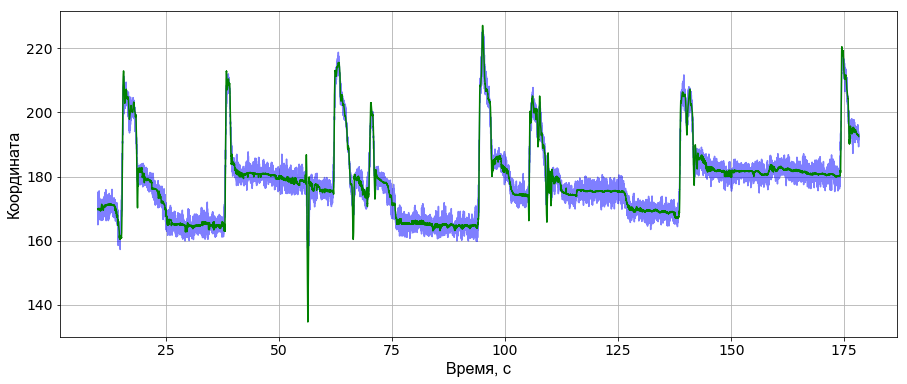
\includegraphics[width=300pt,height=\textheight,keepaspectratio]{imgs/motrenko-train.png}
	\caption{Результаты работы PLSRegression на предобработанных данных, тренировочная выборка}	
	\label{fig:motr train}
	\end{center}
\end{figure}


\begin{figure}
\begin{center}
	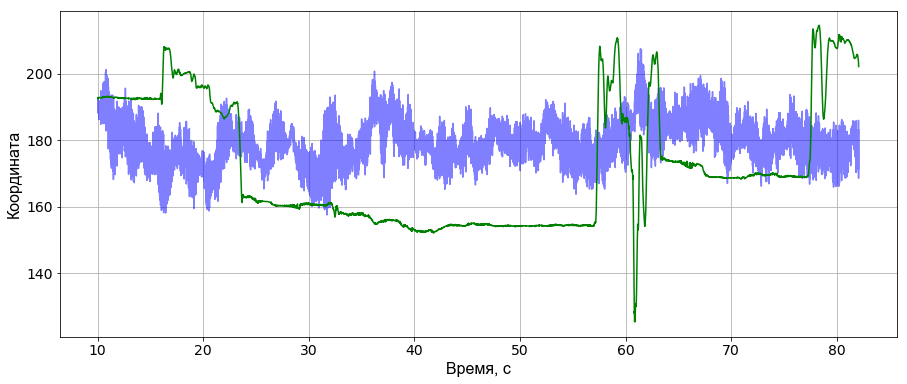
\includegraphics[width=300pt,height=\textheight,keepaspectratio]{imgs/motrenko-test.png}
	\caption{Результаты работы PLSRegression на предобработанных данных, тестовая выборка}	
	\label{fig:motr test}
	\end{center}
\end{figure}


\begin{table}[h]
  
  \centering
    \begin{tabular}{ | c | c | c | c | }
	\hline
	выборка &mae & mse & r2-score \\ \hline
	train &1.69 & 5.38 & 0.96 \\
	test & 5.38 & 472.42& -0.37\\
	\hline
	\end{tabular}
\caption{Метрики для алгортима PLSRegression}
\label{table:motrenko}
\end{table}

\textbf{Можно ещё про простую регрессию  на сырых данных написать}

\section{Методы построения локальных моделей}
Основываясь на существующем представлении о распространении сигнала по нейронам, предполагается, что амплитуда импульса в зависимости от времени имеет форму, похожую на нормальное или гамма распределение. То есть, существует пик, в котором суммарное напряжение максимально. Вокруг этого пика сигнал убывает по координате в соответствии с законом нормального распределения. Таким образом, выдвигаются следующие гипотезы: в каждый момент времени распределение интенсивности сигнала в пространстве каналов имеет нормальное или гамма-распределение. в обоих случаях распределение понимается двумерным. Соответствие пространства каналов координатному представлению представлено на [рис.N] \textbf{нарисую}. Учитывая, что напряжение на каналах может быть как положительным, так и отрицательным, будем также рассматривать параметр пиковой интенсивности и производить домножение на него. Данная поправка масштабирует результат и определяет его знак. 
\subsection{Гипотеза нормального распределения сигнала среди каналов}
\subsubsection{Математическая постановка} 
Интенсивность сигнала подчиняется модели нормального распределения: $\mathbf{x}_t \in \mathcal{N}(\mathbf{m}(t),\mathbf{\sigma}(t))$. Математическое ожидание $\mathbf{m}(t)$ аппроксимирует положение пика интенсивности в момент времени $t$, а ковариационная матрица $\mathbf{\sigma}(t)$ описывает форму фронта. Параметры распределения $\mathbf{\theta}$ = ($\mathbf{m}(t), \mathbf{\sigma(t)}$).
\subsubsection{Эксперименты}
Сначала рассмотрим, можно ли восстановить электрокортикограмму, пользуясь локальной моделью. Хорошее качество восстановления исходных данных по модели позволило бы считать локальную модель заведомо удачной..

\begin{figure}
\begin{center}
	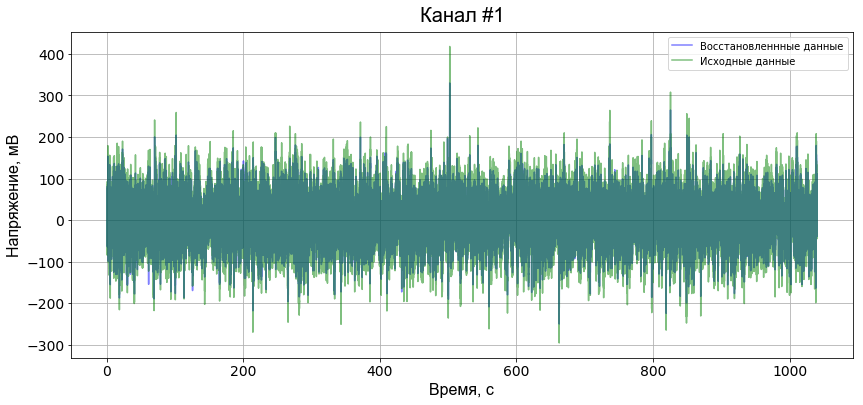
\includegraphics[width=300pt,height=\textheight,keepaspectratio]{imgs/Gauss_ch1.png}
	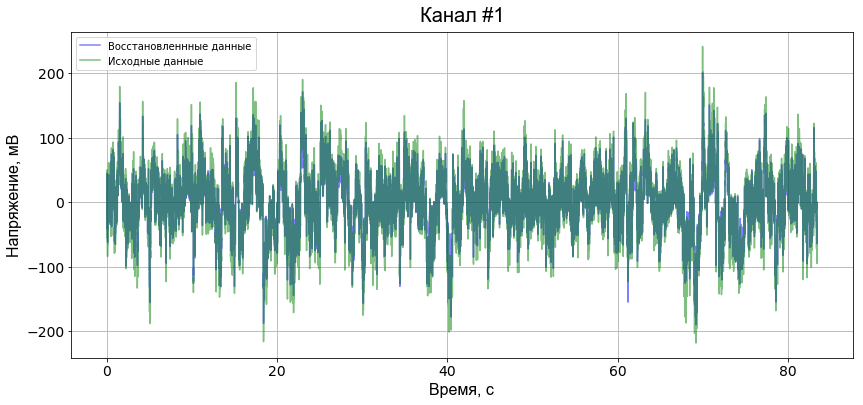
\includegraphics[width=300pt,height=\textheight,keepaspectratio]{imgs/Gauss_ch1_80s.png}
	\caption{Восстановление эког по нормальному распределению, 1 канал}	
	\label{fig:gauss ecog}
	\end{center}
\end{figure}


Значения метрик:
\begin{table}[h]
  
  \centering
    \begin{tabular}{ | c | c | c | }
	\hline
	mae & mse & r2-score \\ \hline
	90.69 & 22129.04 & -0.05 \\

	\hline
	\end{tabular}
\caption{Метрики для гипотезы нормального распределения}
\label{table:gauss mae}
\end{table}

Регрессионная модель, восстанавливающая ECoG по параметрам локальной модели является ненудовлетворительной.
\subsubsection{Выводы}
полученные результаты говорят о том, что предположение о нормальном распределении сигнала в пространстве является ошибочным как с нормировкой на интенсивность, так и без неё. Однако пиковая интенсивность дает достаточно хорошее описание электрокортикограммы. 
\subsection{Гипотеза гамма-распределения}

\subsubsection{Математическая постановка} 
Если предположить дополнительно, что на распределение интенсивности в пределах группы нейронов влияет направленное распространение сигнала внутри группы, можно выдвинуть гипотезу $x_{ti}
\in \Gamma(k, \theta)$, $i=1,\dots,N$, так как гамма-распределение не является симметричным. Параметры распределения $\mathbf{\theta}$ = $\{(k_i$, $\theta_i)\}_{i=1}^T$. 
\subsubsection{Эксперименты}
Также сначала рассмотрим качество отображения из нового признакового пространства в исходное. 
\begin{figure}
\begin{center}
	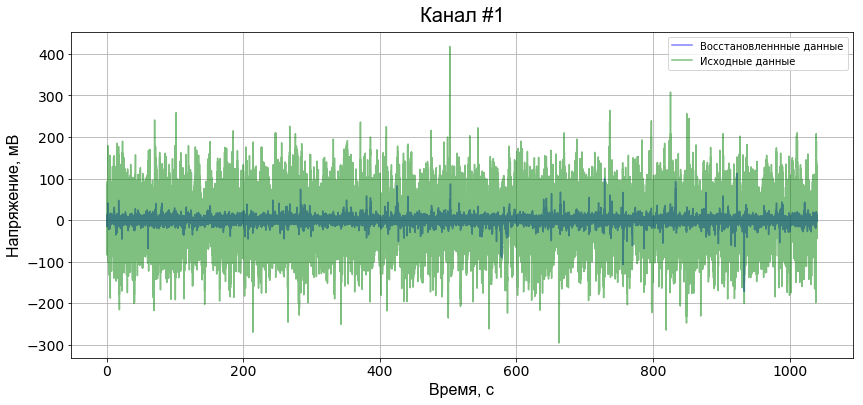
\includegraphics[width=300pt,height=\textheight,keepaspectratio]{imgs/wishart_raw1.png}
	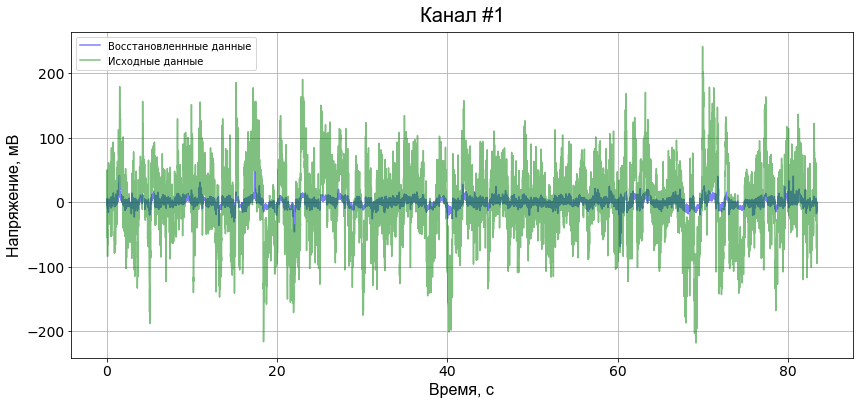
\includegraphics[width=300pt,height=\textheight,keepaspectratio]{imgs/wishart_raw1_80s.png}
	\caption{Восстановление эког по гамма-распределению, 1 канал}	
	\label{fig:gamma ecog}
	\end{center}
\end{figure}


Значения метрик:
\begin{table}[h]
  
  \centering
    \begin{tabular}{ | c | c | c | }
	\hline
	mae & mse & r2-score \\ \hline
	33.76 & 1921.38 & 0.02 \\

	\hline
	\end{tabular}
\caption{Метрики для гипотезы нормального распределения}
\label{table:gauss mae}
\end{table}


Как и в случае с нормальным распределением, модель не даёт положительных результатов.

 
\subsubsection{Результаты точечных локальных моделей}
Рассмотрим модель регрессии, обученную на пяти полученных признаках: мат.ожидание, дисперсия, интенсивность. Восстановим эког по параметам регрессией и случайным лесом. Сравним получившиеся модели:

\begin{figure}
\begin{center}
	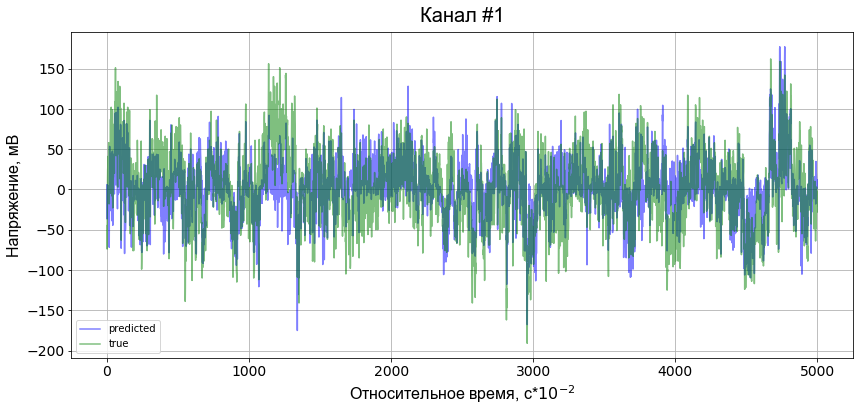
\includegraphics[width=300pt,height=\textheight,keepaspectratio]{imgs/ecog_by_params_lr.png}
	\caption{Восстановление эког по параметрам распределений с помощью линейной регресиии, 1 канал}	
	\label{fig:lr ecog}
	\end{center}
\end{figure}

\begin{figure}
\begin{center}
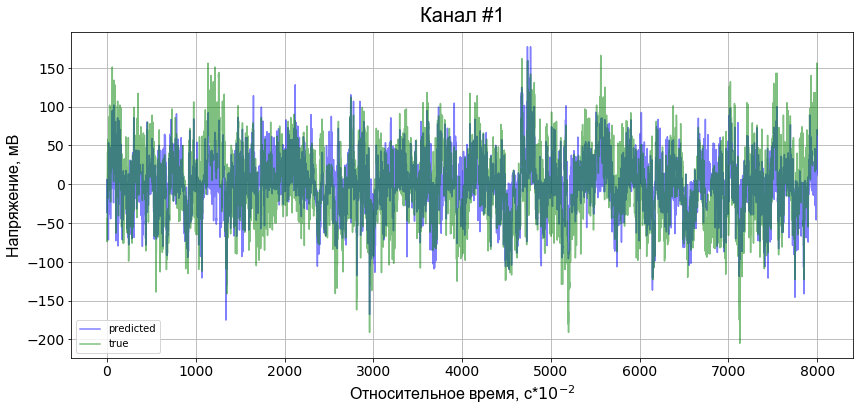
\includegraphics[width=300pt,height=\textheight,keepaspectratio]{imgs/ecog_by_params_rf.png}
\caption{Восстановление эког по параметрам распределений с помощью случайного леса, 1 канал}	
	\label{fig:rf ecog}
	\end{center}
\end{figure}


Значения метрик:
\begin{table}[h]
  
  \centering
    \begin{tabular}{ | c | c | c | c | }
	\hline
	модель&mae & mse & r2-score \\ \hline
	Линейная регрессия &34.67 & 2117.99 & 0.11 \\
	Random forest &31.29 & 1814.65 & 0.26\\
	\hline
	\end{tabular}
\caption{Метрики для гипотезы нормального распределения}
\label{table:lr/rf ecog}
\end{table}
Попробуем по этим параметрам восстановить движение:

\begin{figure}
\begin{center}
	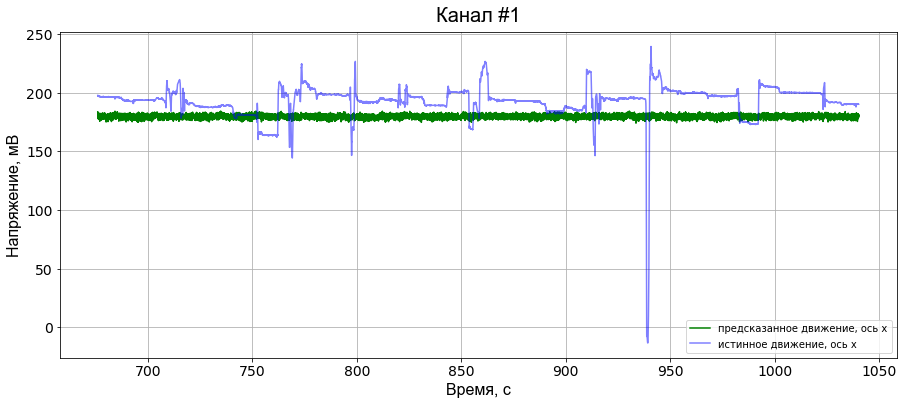
\includegraphics[width=300pt,height=\textheight,keepaspectratio]{imgs/motion_by_params.png}
	\caption{Восстановление движения по параметрам модели}	
	\label{fig:motion gauss}
	\end{center}
\end{figure}

Значения метрик:
\begin{table}[h]
  
  \centering
    \begin{tabular}{ | c | c | c | }
	\hline
	mae & mse & r2-score \\ \hline
	26.85 & 1479.59 & -0.28 \\

	\hline
	\end{tabular}
\caption{Метрики для предсказания}
\label{table:gauss mae}
\end{table}
Полученная модель не превосходит по качеству заданные базисные уровни.
\subsubsection{Выводы}
полученные результаты говорят о том, что предположение об экспоненциальном распределении сигнала в пространстве является ошибочным. 

\section{Генерация признаков}

\section{Временные отрезки}

\chapter{Результаты}
%В ходе исследования был проведен ряд экспериментов. Результаты показали, что локальные модели ... не имеют достаточной сложности для описания исследуемых явлений.
%Локальная модель...хорошая потому что.
%Результаты исследований. Интерпретация результатов. Обоснование достоверности и оценка их соответствия поставленным задачам

%Указать результативность каждого из методов в r2-score, mae. Сравнить raw, предобработку как на рез-т так и на время.


%Рекомендации по дальнейшему использованию
\chapter{Заключение}
%Обобщение рез-тов работы, план дальнейших действий
%Исследование
В результате данной работы построены несколько локальных моделей, дающих приемлемое качество последующих предсказаний движения. Предполагается дальнейшее улучшение этих моделей, а также использование их результатов в качестве baseline для построения более удобного признакового пространства с ипользованием алгоритмов глубокого обучения.



% Следующие строки необходимо раскомментировать, а предыдущую закомментировать, если используется inline-библиография.
%\begin{thebibliography}{99}
%    \bibitem{langmuir26}
%        H. Mott-Smith, I. Langmuir. ``The theory of collectors in gaseous discharges''. \emph{Phys. Rev.} \textbf{28} (1926)
%\end{thebibliography}


\end{document}